\section{Symmetric key Encryption - AES}

Symmetric key encryption use the same key for both encryption and decryption. It's the most intuitive form of encryption. There are lots of algorithms for symmetric encryption, but the most typical is \textbf{AES (Advanced Encryption Standard).}

AES is a block cipher, which means that it encrypts 128 bits at a time. This means that each number we can have with 128 bits, has a "translation" into the encrypted world, that is 128 bits long too. The key is used to make this translation, and is different for every key used.

If the data we have to encrypt is exatly 128 bits long, this works perfectly, but what happens when data is larger? Then we have to use a \textit{block cipher mode of operation}.

\subsection{Block cipher mode of operation}
A mode of operation is an algorithm that explains how to apply a cipher's single-block operation (in this case, AES) to encrypt amounts of data larger than a block. There are many algorithms, but we are only going to explain two of them.

\subsubsection{Electronic Codebook (ECB)}
ECB is the most intuitive mode, but also the most insecure. With this mode of operation, the data is divided between blocks, and then each block is encrypted separately.
\begin{figure}[htb]
	\begin{centering}
		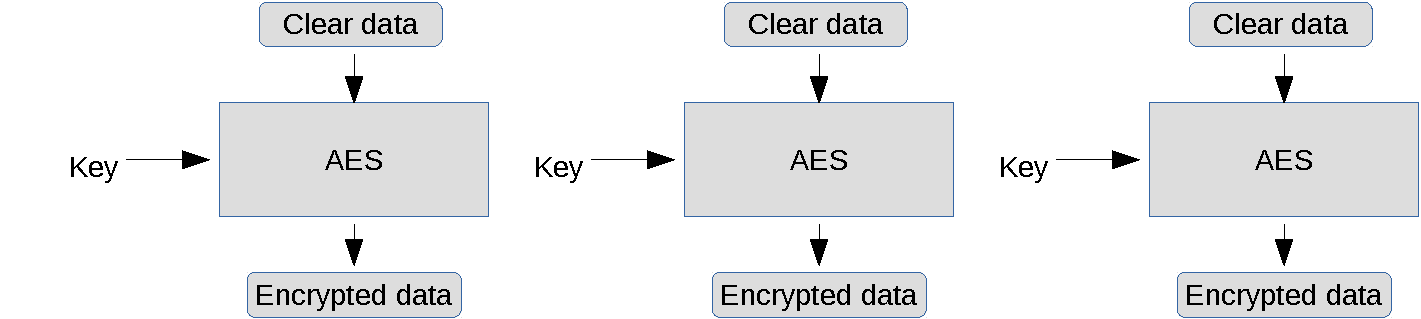
\includegraphics[width=0.7\columnwidth]{\securitydir/basicJsCrypto/figures/ecb}
		\par\end{centering}
	\caption{\label{fig:ecb} ECB Mode explained}
\end{figure}

ECB is not secure because each block has the same encrypted value so the data itself cannot be retrieved, but the attacker can recognize patrons in it. For example, if we send a "Hello" at the beginning of the message using ECB, the attacker does not know what's the meaning of it, but he can know every time it is sent.


\subsubsection{Cipher Block Chaining (CBC)}	

In this mode, each block is XORed with the previous block, then encrypted as usual. This way, to decipher a block, we need to decipher all the previous ones

\begin{figure}[htb]
	\begin{centering}
		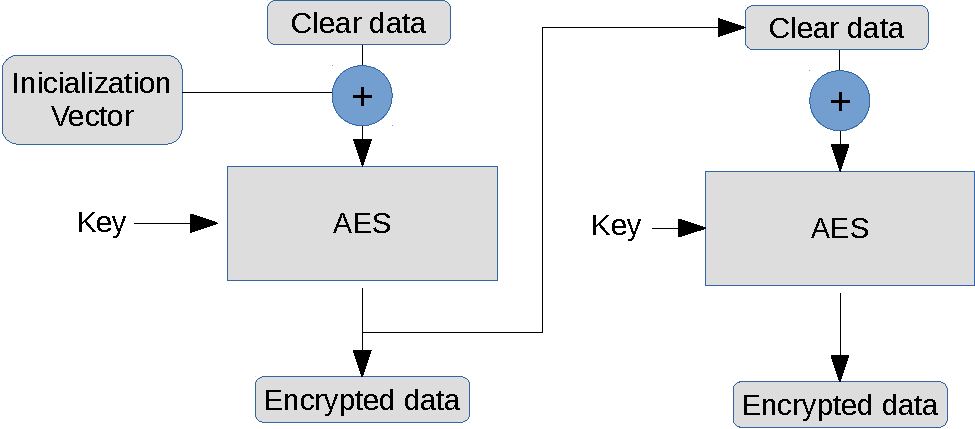
\includegraphics[width=0.7\columnwidth]{\securitydir/basicJsCrypto/figures/cbc}
		\par\end{centering}
	\caption{\label{fig:cbc} CBC Mode explained}
\end{figure}

\subsection{NodeJS tips}
If we go to the crypto library documentation (\url{https://nodejs.org/api/crypto.html}), there are two implementations proposed. The first one is intended to be used when the data to be encrypted has a determined length.

\begin{js}
const crypto = require('crypto');
const cipher = crypto.createCipher('aes192', 'a password');

let encrypted = cipher.update('some clear text data', 'utf8', 'hex');
encrypted += cipher.final('hex');
console.log(encrypted);
\end{js}

The second implementation uses NodeJS \textbf{Streams}. Streams are objects that can be read and written to. If we use the cipher as a stream, we can write the clear data to it, and then read the encrypted data. What makes streams very useful is that they can be piped to each other, thus making the write method redirect automatically to the input of another stream. This way we can input the data to be ciphered indefinitely until closed.

\begin{js}
const crypto = require('crypto');
const fs = require('fs');
const cipher = crypto.createCipher('aes192', 'a password');

const input = fs.createReadStream('test.js');
const output = fs.createWriteStream('test.enc');

input.pipe(cipher).pipe(output);
\end{js}